%%%%%%%%%%%%%%%%%%%%%%%%%%%%%%%%%%%%%%%%%%%%%%%%%%%%%%%%%%%%%%%%%%%%%%%%%%%%%%%%%%%%
% Document data
%%%%%%%%%%%%%%%%%%%%%%%%%%%%%%%%%%%%%%%%%%%%%%%%%%%%%%%%%%%%%%%%%%%%%%%%%%%%%%%%%%%%
\documentclass[12pt]{article} %report allows for chapters
%%%%%%%%%%%%%%%%%%%%%%%%%%%%%%%%%%%%%%%%%%%%%%%%%%%%%%%%%%%%%%%%%%%%%%%%%%%%%%%%%%%%
\usepackage{preamble}

\newcommand{\curvegamma}{\boldsymbol{\vec{\gamma}}}
\newcommand{\tangentgamma}{\boldsymbol{\dot{\vec{\gamma}}}}
\newcommand{\normalgamma}{\boldsymbol{\ddot{\vec{\gamma}}}}
\newcommand{\vecfieldB}{\boldsymbol{\vec{B}}}
\newcommand{\vecfieldJ}{\boldsymbol{\vec{J}}}
\newcommand{\vecfieldF}{\boldsymbol{\vec{F}}}
%\newcommand{\vecfieldE}{\boldsymbol{\vec{E}}}
\newcommand{\vecx}{\boldsymbol{\vec{x}}}
\usepackage{subcaption}
\usepackage{caption}
\begin{document}

\begin{center}
   \textsc{\large MATH 272, Homework 2}\\
   \textsc{Due February 11$^\textrm{th}$}
\end{center}
\vspace{.5cm}


\begin{problem}
\textbf{(6 pts.)} Here is a plot of a 3-dimensional vector field $\vecfieldV$ when viewing from a few different angles.
\begin{figure}[H]
    \centering
    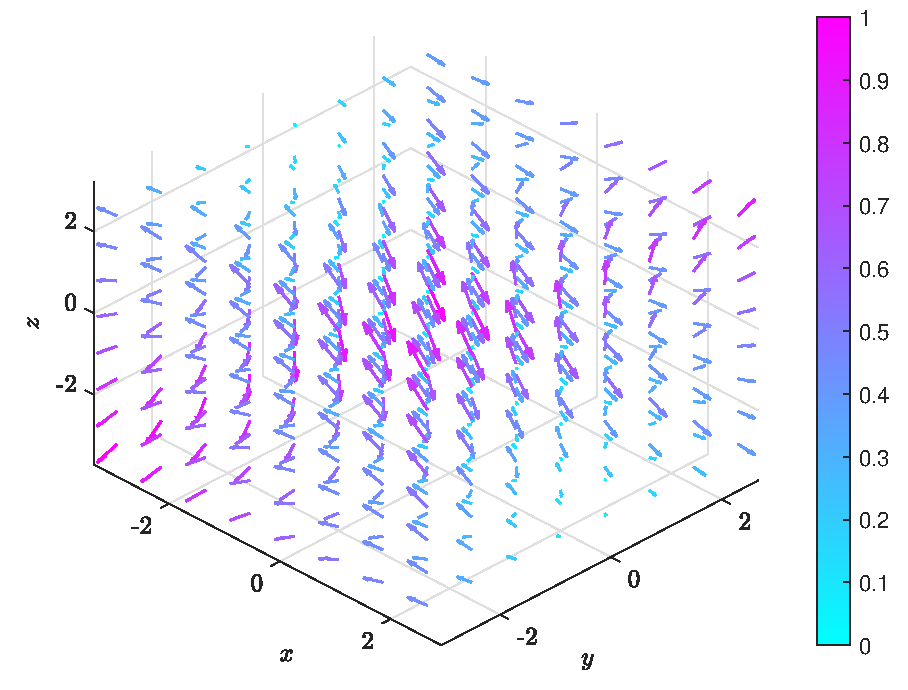
\includegraphics[width=.85\textwidth]{figures/vecfield}
    \caption{A view of the vector field $\vecfieldV$. Note that the colorscaling on this plot represents the length of the vectors. The next plots use the same colorscale.}
\end{figure}
\begin{figure}[H]
    \centering
    \begin{subfigure}[b]{0.45\textwidth}
        \centering
        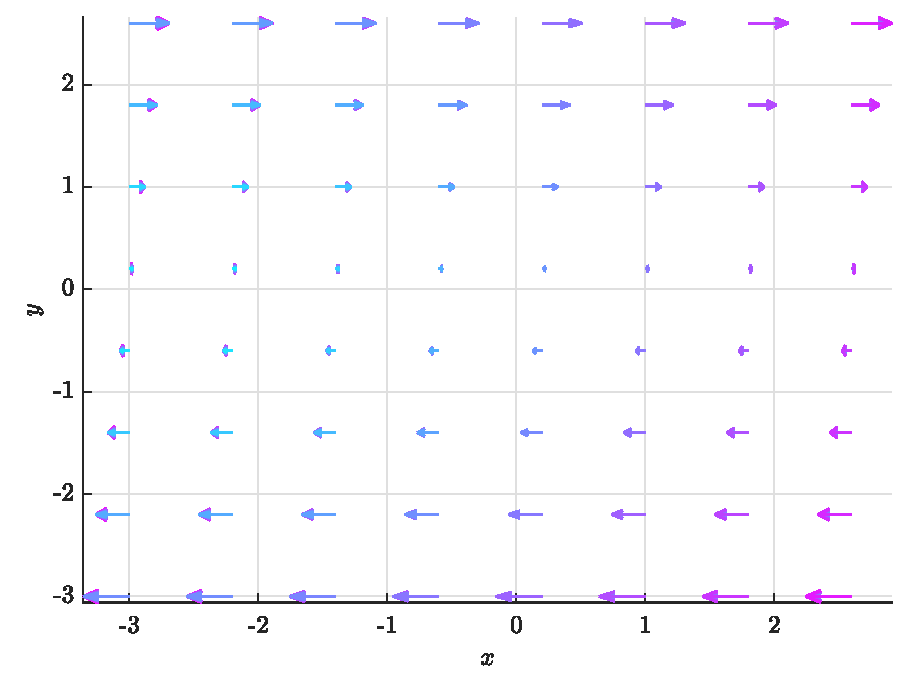
\includegraphics[width=\textwidth]{figures/vecfield_xy}
        \caption{$\vecfieldV$ when looking towards the $xy$-plane.}
    \end{subfigure}
    \quad
    \begin{subfigure}[b]{0.45\textwidth}
        \centering
        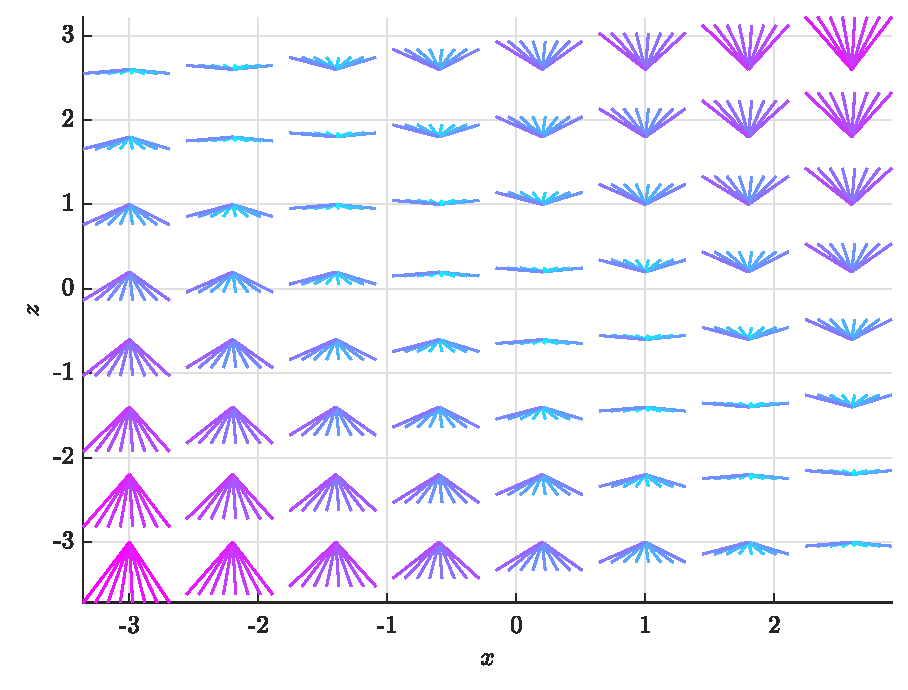
\includegraphics[width=\textwidth]{figures/vecfield_xz}
        \caption{$\vecfieldV$ when looking towards the $xz$-plane.}
    \end{subfigure}
\end{figure}
\begin{enumerate}[(a)]
    \item \textbf{(3 pts.)} Does this vector field have divergence? Explain.
    \item \textbf{(3 pts.)} Does this vector field have curl? Explain.
\end{enumerate}
\end{problem}

\vspace*{0.5cm}

\begin{problem}
\textbf{(8 pts.)} Consider the vector field
\[
\vecfieldV(x,y,z) = \begin{pmatrix} -y \\ x \\ z \end{pmatrix}.
\]
\begin{enumerate}[(a)]
    \item \textbf{(2 pts.)} Compute the Jacobian (or derivative) of $\vecfieldV$.
    \item \textbf{(2 pts.)} Compute the divergence of $\vecfieldV$.
    \item \textbf{(2 pts.)} Compute the curl of $\vecfieldV$.
    \item \textbf{(2 pts.)} Compute the directional derivative of $f$ at $\vecx_0 = (1,2,-3)$ in the direction of $\vecfieldV(\vecx_0)$.
\end{enumerate}
\end{problem}

\vspace*{0.5cm}

\begin{problem}
\textbf{(8 pts.)} Consider the following vector field
\[
\vecfieldB = -\frac{y}{2}\xhat + \frac{x}{2}\yhat.
\]
Here, $\vecfieldB$ denotes the magnetic field. It may be helpful to plot the fields in this problem.
\begin{enumerate}[(a)]
    \item \textbf{(1 pts.)} Show that $\vecfieldB$ has no divergence. (This is one of Gauss's laws.)
    \item \textbf{(1 pts.)} Show that $\grad \times \vecfieldB = \vecfieldJ$ (Amp\'ere's law) where
    \[
    \vecfieldJ = \zhat.
    \]
    This vector field $\vecfieldJ$ represents the electric current (moving charges) in space. One could argue that the current creates the magnetic field via Amp\'ere's law.
    \item \textbf{(4 pts.)} Magnetic fields induce a force $\vecfieldF$ on charged particles by the Lorentz force
    \[
    \vecfieldF = \tangentgamma \times \vecfieldB = \normalgamma
    \]
    Where $\tangentgamma$ is the velocity of the particle (where we have chosen a mass $m=1$ and charge $q=1$).  Let us do the following.
    \begin{itemize}
        \item Assume that $\tangentgamma = \xhat$, what is the force on the particle?
        \item Repeat the previous step for $\tangentgamma=\yhat$ and $\tangentgamma=\zhat$.
        \item Compare and contrast the forces you found.
    \end{itemize}
    \item \textbf{(2 pts.)} Can you argue why applying a magnetic field to a molecule may cause it to heat up? Can you compare this idea with your home microwave?
\end{enumerate}
\end{problem}

\vspace*{0.5cm}

\begin{problem}
\textbf{(6 pts.)} Consider the function
\[
f(x,y)=\sin\left(\frac{2\pi x}{5}\right)\sin\left(\frac{2\pi y}{5}\right).
\]
comes up when you want to find out how a square shaped drum head will vibrate when hit.
\begin{enumerate}[(a)]
    \item \textbf{(1 pts.)} Plot this function on the region $\Omega$ given by $0\leq x \leq 5$ and $0\leq y \leq 5$.
    \item \textbf{(2 pts.)} What is the value the function $f(x,y)$ on the boundary of the given region $\Omega$ (i.e, when $x=0$, $x=5$, $y=0$, and $y=5$)?
    \item \textbf{(3 pts.)} Show that $f(x,y)$ is an eigenfunction of the Laplacian $\Delta$. That is, $\Delta f = \lambda f$ for some eigenvalue $\lambda$. What is the eigenvalue?
\end{enumerate}
\end{problem}

\vspace*{0.5cm}

\begin{problem}
\textbf{(12 pts.)} For the following, describe the composite function as a function $\R^m \to \R^n$, in other words, what is the dimension of the domain and codomain? Then, compute the composite function given to you and write down if there are any other possible composite functions you could make. Finally, what are the dimensions of the matrix that correspond to the derivative of the composite function?
\begin{enumerate}[(a)]
\item \textbf{(4 pts.)} Take $f\colon \R^2 \to \R$ given by $f(x,y)=\sin(xy)$ and let $\curvegamma \colon \R \to \R^2$ be given by $\curvegamma(t) = \begin{pmatrix} t \\ 1 \end{pmatrix}$. The composite function $f\circ \curvegamma$.
\item \textbf{(4 pts.)} Take $\vecfieldV \colon \R^2 \to \R^2$ by $\vecfieldV(x,y)= \begin{pmatrix} xy \\ x+y \end{pmatrix}$ and let $\curvegamma \colon \R \to \R^2$ by $\curvegamma(t) = \begin{pmatrix} \cos(t) \\ \cos^2(t) \end{pmatrix}$. The composite function $\vecfieldV \circ \curvegamma$.
\item \textbf{(4 pts.)} Take $\vecfieldV \colon \R^3 \to \R^3$ by $\vecfieldV(x,y)= \begin{pmatrix} xz \\ yz \\ z^2 \end{pmatrix}$ and let $f \colon \R^3 \to \R$ by $f(x,y,z) = xz + yz + z^2$. The composite function $f\circ \vecfieldV$.
\end{enumerate}
\end{problem}

\vspace*{0.5cm}

\begin{problem}
\textbf{(12 pts.)} Set up but do not compute the integrals of the given fields over the given curves.
    \begin{enumerate}[(a)]
        \item \textbf{(3 pts.)} $f(x,y) = xe^{x+y}+\cos(xy)$, $\curvegamma(t) = \begin{pmatrix} \cos(t) \\ \sin(t) \end{pmatrix}$, $t_0 = 0$, $t_1=2\pi$.
        \item \textbf{(3 pts.)} $g(x,y,z) = \frac{\ln(z^2)}{e^{xy}}$, $\curvegamma(t) = \begin{pmatrix} t \\ t^2 \\ t^3 \end{pmatrix}$ , $t_0 = 1$, $t_1=-1$.
        \item \textbf{(3 pts.)} $\vecfieldU(x,y) = \begin{pmatrix} -y \\ x \end{pmatrix}$, $\curvegamma(t) = \begin{pmatrix} e^t \\ e^t \end{pmatrix}$, $t_0 = 5$, $t_1=10$.
        \item \textbf{(3 pts.)} $\vecfieldV(x,y,z) = \begin{pmatrix} 2x \\ y \\ x \end{pmatrix}$, $\curvegamma(t) = \begin{pmatrix} \cos(t) \\ t \\ \sqrt{t} \end{pmatrix}$, $t_0 = 0$, $t_1=1$.
    \end{enumerate}
\end{problem}

\vspace*{0.5cm}

\begin{problem}
\textbf{(4 pts.)} Let $f(x,y,z)=x \cos(y) + yz$ be a scalar field and let $\curvegamma = \begin{pmatrix} 1 \\ t \\ \sin(t) \end{pmatrix}$ be a curve from time $t_0 = 0$ to $t_1 = 2 \pi$. Compute
\[
    \int_{\curvegamma} f(\curvegamma)d\curvegamma.
\]
\end{problem}

\vspace*{0.5cm}

\begin{problem}
\textbf{(4 pts.)} Show that for any smooth (more than twice differentiable) fields $f(x,y,z)$ and $\vecfieldV(x,y,z)$ that
\begin{enumerate}[(a)]
	\item \textbf{(2 pts.)} $\grad \times \left(\grad f\right)=\boldsymbol{\vec{0}}$;
	\item \textbf{(2 pts.)} $\grad \cdot \left(\grad \times \vecfieldV\right)=0$.
\end{enumerate}
\end{problem}

\vspace*{0.5cm}

\begin{problem}
\textbf{(5 pts.)} Let
	\[
	\vecfieldU(x,y,z) = \begin{pmatrix} -y \\ x \\ 0 \end{pmatrix} \qquad \textrm{and} \qquad \vecfieldV(x,y,z) = \begin{pmatrix} 2x \\ 2y \\ 2z \end{pmatrix},
	\]
	be vector fields.
	\begin{enumerate}[(a)]
		\item \textbf{(1 pts.)} Explain why there exists no potential function $\phi(x,y,z)$ for the vector field $\vecfieldU$.
		\item \textbf{(1 pts.)} Explain why there does exist a potential function $\phi(x,y,z)$ for the field $\vecfieldV$.
		\item \textbf{(3 pts.)} Compute the potential function for $\vecfieldV$.
	\end{enumerate}
\end{problem}

\vspace*{0.5cm}

\begin{problem}
\textbf{(10 pts.)} Consider the following vector field
    \[
    \vecfieldE = \frac{x}{\left(x^2+y^2+z^2\right)^{3/2}} \xhat + \frac{y}{\left(x^2+y^2+z^2\right)^{3/2}} \yhat + \frac{z}{\left(x^2+y^2+z^2\right)^{3/2}} \zhat,
    \]
    which you can think of as the electric field of a positive point charge.  It turns out that this field $\vecfieldE$ is conservative (which you will show in (a)). Specifically, $\vecfieldE = \grad \phi$, for the scalar field
\[
\phi(x,y,z) = \frac{1}{\sqrt{x^2+y^2+z^2}}
\]
This is Faraday's law for static fields.
    \begin{enumerate}[(a)]
        \item \textbf{(2 pts.)} Compute the divergence and curl of $\vecfieldE$. What can we say about the vector field, its divergence, and its curl at the origin?
        \item \textbf{(3 pts.)} Compute the integral
        \[
        T=\int_{\curvegamma} \vecfieldE \cdot d\curvegamma \qquad \textrm{where} \qquad \curvegamma(t) = \begin{pmatrix} t \\ t \\ t \end{pmatrix},
        \]
        and $t\in [t_0,t_1]$ with $t_0$ and $t_1$ both greater than 0.  Note that this integral $T$ describes the gain in kinetic energy of a charged particle that moved along the path $\curvegamma$.
        \item \textbf{(3 pts.)} Equivalently, since $\vecfieldE$ is conservative, we have
        \[
        T=\int_{\curvegamma} \vecfieldE \cdot d\curvegamma = \phi(\curvegamma(t_1))-\phi(\curvegamma(t_0)).
        \]
        Show that this is true for the given vector field and potential. This shows that the choice of path does not matter; only the endpoints $\curvegamma(t_0)$ and $\curvegamma(t_1)$ matter.
        \item \textbf{(2 pts.)} Argue why the integral around any closed curve must be zero.
    \end{enumerate}
\end{problem}

%\vspace*{0.5cm}
%
%\begin{problem}
%Consider the two dimensional scalar field $T(x,y)=x+y$ that describes the temperature on the square plate $\Omega$ given by the set $0\leq x,y \leq 1$.  Compare the two answers you get!
%\begin{enumerate}[(a)]
%	\item Compute the integral
%	\[
%	\int_\Omega T d\Omega.
%	\]
%	\item Let $\curvegamma$ be the curve that traverses the boundary of the square plate in the counterclockwise direction.  Compute
%	\[
%	\int_{\curvegamma} T d\curvegamma.
%	\]
%\end{enumerate}
%\end{problem}

\vspace*{0.5cm}

\begin{problem}
\textbf{(3 pts.)} Let $f(x,y,z)=2xy+e^{xz}+\sin(y)$ be a scalar field. Integrate $f$ over the triangular prism $\Omega$ defined by taking the half triangle of the unit square in the $xy$-plane satisfying $x\leq y$ and with height 4 above the $xy$-plane.
\end{problem}


\end{document}